%!TEX root = tesi.tex

\chapter{Four dimensional dualities}

%!TEX root = tesi.tex
\begin{lstlisting}
---- INTRODUCTION OUTLINE-----
~ More symmetry = more tools for studying t\heories
~ Milder divergences 
~ Renormalization constraints
~ Non renormalization theorems (perturbative)
~ Holomorphicity, couplings as background fields 
~ Exact results (superpotential, exact beta function )
~ Moduli space
\end{lstlisting}





\section{Introduction}
Supersymmetric quantum field theories enjoy an enlarged group of  symmetries compared to other field theories. 
Since the symmetry group is a non trivial combination of internal and spacetime symmetries, they have many unexpected features and new techniques were found to study them.
Almost all of the new tools found are available only for supersymmetric field theories, making them the theater for many advances in physics. 

A more technical introduction on supersymmetry and its representation on fields can be found in appendix \ref{appendice_susy}.

In this section we will analyse more advanced features of supersymmetric field theories that has been used intensively in the discovery and in the analysis of electric magnetic duality and its generalisations.













\subsection{General renormalization properties}

A remarkable feature of supersymmetry is the constraint that the additional symmetry imposes on the renormalization properties of the theories.

One of the first aspects that brought attention to supersymmetry was that divergences of loop diagrams were milder because of the cancellation between diagrams with bosons and fermions running in the loops. 

Nowadays we know powerful theorems that restrict the behaviour of supersymmetric field theories during renormalization.
In order to preserve supersymmetry, the renormalization process has to preserve the Hilbert space structure. For example the wave function renormalization of different \emph{particles} inside a multiplet must be the same, otherwise the renormalized lagrangian is not supersymmetric invariant anymore. 

Moreover, in the supersymmetry algebra $P^2$ is still a Casimir operator i.e. it commutes with every operator in the algebra: particles in the same multiplet must have the same mass.
Renormalization cannot break this condition, otherwise it would break supersymmetry.

For a \emph{Super Yang Mills} theory with $\mathcal{N} = 1$ we have the additional requirement that $g V$, where $g$ is the coupling and $V$ is the vector superfield, cannot be renormalized by symmetry considerations. 
%This is equivalent to require that  $ Z_g = Z_V^{-1}$.

Adding more supersymmetry the wave function renormalization of the various field are even more constrained by symmetry.
For example, for $\mathcal{N}=4$ \emph{SYM} the fields and the coupling are not renormalized at all.








\subsubsection{Beta function for SYM and SQCD}
Another nice feature of supersymmetric field theories is that some quantities can be calculated exactly.
The first object of this kind that we encounter is the $\beta$ function of four dimensional $\mathcal{N} =  1 $ \emph{Super Yang Mills} and \emph{Super QCD} theories.

It is given by the \emph{NSVZ $\beta$ function} 
\begin{equation}
  \beta (\alpha) = - \frac{\alpha^2}{2 \pi} \left[ 3 \; T(Adj) - \sum_i T( R_i) ( 1 - \gamma_i ) \right]  \left( 1 - \frac{ \alpha \; T(Adj)  }{2 \pi} \right)^{-1} \qquad \alpha = \frac{g^2}{4 \pi}
\label{beta-exact}
\end{equation} 
where $\gamma_i$ are the anomalous dimensions of the matter fields and $T(R_i)$ are the dynkin indices of their representation.\\
The anomalous dimensions are defined as
\begin{equation}
 \gamma_i = - \frac{d \, \log(Z_i) }{d \, \log( \mu)}
\end{equation}
where $Z_i$ is the wave function renormalization coefficient.
For example for gauge group $SU(N)$ we have
\begin{equation*}
 T(N) = \frac{1}{2} \qquad T(Adj) = N 
\end{equation*}
The \emph{NSVZ $\beta$ function} was first calculated using instanton methods in \cite{Novikov:1985rd}. 
Over the years it has been calculated in other ways using the fact that the action is holomorphic in the complexified coupling
\begin{equation}
	\frac{1}{g_h^2} = \frac{4 \pi i }{g_c^2 } + \frac{\theta_{YM}}{2 \pi} 
\end{equation}
Using the holomorphic coupling the action for the vector field is written as
\begin{equation}
 \mathcal{L}_h ( V_h) = \frac{1}{32 \pi i } \int d^2 \theta \frac{1}{g_h^2} W^a ( V_h) W^a(V_h)  + h.c.
\end{equation}
whereas with the canonical normalization for the vector field is
\begin{equation}
 \mathcal{L}_c ( V_c) = \frac{1}{32 \pi i } \int d^2 \theta \left( \frac{4 \pi i }{g_c^2 } + \frac{\theta_{YM}}{2 \pi} \right) W^a ( g_c V_c) W^a(g_c V_c) + h. c.  
\end{equation}
Using the canonical normalization $g_c V_c$ is a real superfield, imposing that $g_c$ is real.
For this reason with the canonical normalization the lagrangian is not holomorphic in the combination $ \frac{1}{g^2 } + i \frac{\theta}{8 \pi^2} $.
Thanks to holomorphy, the holomorphic coupling is only renormalized at one-loop and the $\beta$ function can be computed but its expression is different from \emph{NSVZ $\beta$ function}.
In fact, the \emph{NSVZ $\beta$ function} is defined using the canonical (or physical) coupling constant and receives contribution from all orders in perturbation theory.

At first sight, one should expect that the expressions should match since the first two orders in $\alpha$ of the $\beta$ function are scheme independent. 
The reason why the two expressions differ is that the Jacobian of the transformation between canonical and holomorphic normalization is anomalous. 
Once the anomaly is taken into account the two expressions for the $\beta$ function agree. 
An explicit calculation relating the comparison between the two different approach can be found in \cite{ArkaniHamed:1997mj}.










\subsection{Superpotential: holomorphy and non-renormalization}
Other than renormalization constraints, supersymmetry provides non-renormalization theorems for certain objects, such as the superpotential.
In \cite{Grisaru:1979wc} it has been demonstrated that the superpotential is tree-level exact, i.e. it does not receive correction in perturbation theory. 
However it usually receive contributions from non perturbative dynamics.

Perturbative calculations can be done using supergraphs, i.e. Feynman diagrams with superfields. 
The advantage of this approach is that supersymmetry is explicit and many semplification occur naturally. 
The demonstration is based on the fact that for general supersymmetric field theories, supergraph loops diagrams yield a term that can be written in the form
\begin{equation}
\int  d^4 x_1 \dots d^4 x_n d^2 \theta d^2 \bar{\theta} \; G (x_1 , \dots , x_n) \,F_1 ( x_1, \theta, \bar{\theta}) \dots  F_n ( x_n, \theta, \bar{\theta}) 
\end{equation} 
where $G (x_1 , \dots , x_n) $ is translationally invariant function.\\
The importance of this result is that all contribution from Feynman diagrams are given by a single integral over full superspace ($d^2 \theta d^2 \bar{\theta} $) whereas the superpotential must be written as an integral in half-superspace($d^2 \theta $ only) of chiral fields.
Exploiting the fact that a product of chiral fields is a chiral field, the most general form of a superpotential is 
\begin{equation}
 W (\lambda, \Phi) = \sum_{n=1}^{\infty} \left( \int d^2 \theta \, \lambda_n \Phi^n  \; +\;  \int d^2 \bar{\theta} \, \lambda_n^{\dagger} \bar{\Phi}^n \right)
 %\int d^2 \bar{\theta} \bar{\lambda}_n {\bar{\Phi}}^n
 \end{equation} 
 The second term of the superpotential is added in order to give a real lagrangian after the integration in superspace.
From the definition, we can see that the superpotential is holomorphic in the fields and in the coupling constants.

Fifteen years later, Seiberg \cite{Seiberg:1993vc} provided a proof of this theorem using a different approach.
He noted that the coupling constants $\lambda_n$ can be treated as background fields, i.e. chiral superfields with no dynamics.

Using this observation we can assign transformation laws to the coupling constants, making the lagrangian invariant under a larger symmetry.
Fields and coupling constants are charged under this symmetry and only certain combinations of them can appear in the superpotential.
%The superpotential in the weak coupling limit is subject to the constraints imposed by holomorphy and symmetry.
In addition, in a suitable weak coupling limit the effective superpotential must be identical with the tree-level one.
These conditions, taken together, fix the expansion of the superpotential to the expression of the tree-level potential.
A more detailed discussion can be found in \cite{Seiberg:1994bp} and \cite{Intriligator:1995au}.











\subsection{Moduli space}
Supersymmetric field theories have a larger set of vacua compared to ordinary field theories because of the presence of many scalar fields in the supermultiplets.

Lorentz invariance of the vacuum forbids fields with spin different from zero to acquire a vacuum expectation value.
With the same reasoning, derivatives of scalar fields must be set to zero because of translational invariance of the vacuum.
The scalar potential is the only term in the Lagrangian and in the Hamiltonian that can differ from zero.
As a result, the minimums of the scalar potential are in one-to-one correspondence with the states of minimal energy of the theory.


For $4D \; \mN=1$ gauge theories with matter, the scalar potential (involving only squarks in this case) is given by
\begin{equation}
 V ( \phi_i, \bar{\phi}_j) = F \bar{F} + \frac{1}{2} D^2  \quad \overset{\mathclap{on-shell}}=   \quad \frac{\partial W}{\partial \phi_i} F^i \frac{\partial \bar{W}} {\partial \bar{\phi}_i} \bar{F}^i + \frac{g^2}{2} \sum_a | \bar{\phi}_j (T^a)^j_i \phi^j + \xi^a | ^2  \geq 0
\end{equation} 
$\xi^a$ is the Fayet-Iliopulos coefficient and differs from zero only for abelian factors of the gauge group.
The last equality is valid since $D$ and $F$ are auxiliary scalar field of vector and chiral fields respectively.
Their value is set by their equations of motion
\begin{equation}
 \bar{F}_i  = \frac{\partial \bar{W}} {\partial \bar{\phi}_i} \qquad D^a = - g \bar{\phi} T^a \phi - g \xi^a 
\end{equation}
Supersymmetric vacua are described by the sets of values of the scalar \emph{VEVs} that give a zero scalar potential. 
This requirement is equivalent to two different sets of equations, called $D-term$ and $F-term $ equations
\begin{equation}
\bar{F}^i ( \phi) = 0 \qquad D^a (\phi , \bar{\phi}) = 0
\end{equation}
\emph{F-term} equations are present only if there is a superpotential.

Some theories do not have supersymmetric vacua and in these cases supersymmetry is spontaneously broken. 

The \emph{classical moduli space} is the set of solution of these equations for scalar \emph{VEVs} and represents the classical supersymmetric vacua of the theory. 
Gauge transformation should be taken into account in order to avoid redundance in the description.
The moduli space describe physically inequivalent vacua, since the mass spectrum of the theory depends on the \emph{VEVs} of the scalar fields, that differ in every point of the moduli space. 

Thanks to supersymmetry radiative corrections do not lift the energy of the ground state and the vacuum remains supersymmetric.
Only superpotentials generated from non perturbative dynamics can lift the moduli space. 
We will see examples of this phenomenon in the analysis of SQCD.

An alternative description of the space of classical \emph{D-flat} directions is given by the space of all holomorphic gauge invariant polynomials of scalar fields modulo classical relations between them \cite{Luty:1995sd}. 
If a superpotential is present, \emph{F-term} equations should be imposed on the gauge invariant polynomial used to describe \emph{D-flat} direction.
We will use this convenient description in the next chapters.



\subsubsection{Moduli space of $4D \; \mN=1$ SQCD with $SU(N_c)$ gauge group and $N_f$ flavors}
As a concrete example of moduli space we will analyse $SU(N_c)$ SQCD with $N_f$ flavors.
Its classical lagrangian contains no superpotential and is given by two terms, generating \emph{D-terms} equations
\begin{equation}
\mathcal{L } =  \mathcal{L }_{SYM} + \mathcal{L }_{matter} 
\end{equation}
we refer to appendix \ref{appendice_susy} for their explicit form.

The global non anomalous symmetry group of the theory is $SU(N_f)_L \times SU(N_f)_R \times U(1)_B \times U(1)_R$. 
The matter content of the theory consists of $N_f$ $(Q_i, \tilde{Q}^{\tilde{j}})$ pairs of chiral fields, charged under \emph{left}  \emph{right} flavor symmetries respectively. 







\section{Seiberg duality}
\label{sec:seiberg_duality_4d}
Electric magnetic duality relates the dynamics of two different gauge theories in their infrared fixed point.
Even though the dual theories have different particle content, they describe the same IR physics. 
Moreover, whenever one of the dual theories gets more strongly coupled, the other becomes more weakly coupled.
This is particularly useful because it provides an alternative, weakly coupled description of the original theory.




\subsection{Electric theory: $SU(N)$ SQCD with $N_f$ flavours }
We will start our analysis on eletric-magnetic duality studying the first pair of theories that were discovered to be dual in \cite{Seiberg:1994pq}.  
We are going to analyse the properties of these theory in order to better understand the features of the duality.
\\
The electric theory is a $SU(N_c) $ supersymmetric gauge theory with $N_f$ massless flavours.
Its non-anomalous global symmetry group is 
\begin{equation}
SU(N_f)_L \times SU(N_f)_R \times U(1)_B \times U(1)_R 
\label{eqn:seib_dual_global_symm_group}
\end{equation}
The axial symmetry gives rise to an anomaly through the triangular graph $U(1)_A  \times SU(N_c)^2$, hence it is not a symmetry of the theory.\\ 
The classical lagrangian in superspace language is given by
\begin{equation}
 \mathcal{L} = \tau \int d^2 \theta \; Tr ( W_{\alpha} W^{\alpha} ) + \mathrm{h.c.} + 
 \int d^2 \theta \, d^2 \bar{\theta} \;  ({Q}^{i})^{\dagger} e^{ V} Q_i +
 \int d^2 \theta \, d^2 \bar{\theta} \; ({\tilde{Q}^{\tilde{i}})^{ \dagger}} e^{- V} \tilde{Q}_{\tilde{i}}
 \end{equation} 
$Q$ and $\tilde{Q}$ represent left and right quark superfield respectively.
The charges of the fields are given in the table below.
\begin{equation}
 \begin{array}{| c | c |  c c c c |}
 \hline
 & SU(N_c) & SU(N_f)_L  &SU(N_f)_R   & U(1)_B &  U(1)_R \\
\hline
Q & N_c & N_F & 1   &  1  &  \frac{N_f - N_c}{N_f}  \\
\tilde{Q} &\overbar{N_c}  &  1 & \overbar{ N_F}   & -1   &  \frac{N_f - N_c}{N_f}   \\	 
\hline
 \end{array} 
%	\centering
% \caption{Charges of the electric theory}
 \label{tab:suN_elect_charge}
\end{equation}
The value of the R-charge is fixed by the triangle anomaly $SU(N_c)^2 \, U(1)_R $, which can be calculated by considering diagrams with two exiting gluons and the R-symmetry current inserted in the other vertex.
\begin{figure}
\centering
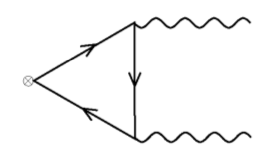
\includegraphics[scale=0.6]{r-symm_anomlay.png}
\label{fig:r_symm_triangle_anom}
\caption{Feynman graphs contributing to the R-symmetry anomaly}
\end{figure}
Each fermion in the theory contributes to the anomaly which, as a result, is proportional to the R-charge of the fermions running in the loop and the Dynkin index of its representation.
Requiring the anomaly to vanish, we find
\begin{align}
R_{gaugino} T (\hbox{Ad}) + \sum_{ f} (& R_{f} - 1)  T(r)   = 0 
\label{eqn:r_symm_anom_condition}
\\
N_c + \frac{1}{2}\,  2 N_f (R_Q -1)  = 0 \quad & \rightarrow \quad R_Q = \frac{N_f - N_c}{N_f}
\end{align}
where we set the gaugino R-charge to $1$ in order to have gluons not charged under R-symmetry.
\\
 The anomaly free condition for the R-symmetry leads to a unique set of R-charges. As a result, we found the R-charges at the superconformal infrared point of the theory.


\subsubsection{Classical moduli space}
Consdering that the theory has no superpotential, the classical moduli space of the theory is given by \emph{D-terms} only. 
They can be read from the on-shell lagrangian and are given by
\begin{equation}
 D^a = g \left( Q^{*i} T^a Q_i - \tilde{Q}^{* i} T^a \tilde{Q}_i \right) = 0
\end{equation}
where $T^a$ are the gauge group generators in fundamental or antifundamental representation and $i$ is a flavour index.
\\
After considering gauge and global symmetries, the squark \emph{VEVs}, represented as $N_f \times N_c$ matrices, which satisfy the D-term equation are given by
\begin{itemize}
\item for $N_f \le N_c$ and $a_i$ generic
\begin{equation}
Q = \tilde{Q} = 
\begin{pmatrix}
 a_1 & 		&	 &	 & \vdots & \vdots \\
	 & a_2  & 	 & 	 & \vdots & \vdots \\  	
 	 & 		&	\ddots &	 &\vdots & \vdots  \\
	 &  & 	 & 	a_{N_f}  & \vdots & \vdots
\end{pmatrix} 
 \\
\end{equation}
\item for $N_f \geq N_c$ and $ | a_i|^2 - | \tilde{a}_i |^2 = a $ independent of $i$.
\begin{equation}
Q  = 
\begin{pmatrix} 
	 a_1 & 		&	 &	  \\
	 & a_2  & 	 & 	 \\  	
 	 & 		&	\ddots &	   \\
	 &  & 	 & 	a_{N_c}  \\
	 \dots & \dots & \dots & \dots\\ 
	 \dots & \dots & \dots & \dots\\ 
\end{pmatrix} 
\quad
\tilde{Q} = 
\begin{pmatrix}
 \tilde{a}_1 & 		&	 &	  \\
	 & \tilde{a}_2  & 	 & 	 \\  	
 	 & 		&	\ddots &	   \\
	 &  & 	 & 	\tilde{a}_{N_c}  \\
	 \dots & \dots & \dots & \dots\\ 
	 \dots & \dots & \dots & \dots\\ 
\end{pmatrix} 
\end{equation}
\end{itemize}
For $N_f \le N_c$ in a generic point of the moduli space the gauge group is broken to $SU(N_c - N_f)$ while for $N_f \geq N_c$ is broken completely.
The gauge group breaks through the super Higgs mechanism: every broken generator is absorbed by the associated massless vector superfield.
This process gives mass to the vector superfield.  
\footnote{Remember that massive representation of supersymmetry have twice the degrees of freedom of massless ones, because in the latter half of the supercharges are represented trivially.}
The mass of the gauge superfield is given by the VEVs of the squarks.
\\
As we said in section \ref{sec:subsection_moduli_space}, we can  study the classical moduli space by finding holomorphic gauge invariant polynomials in the operators and modding out classical relations between them.
For $N_f < N_c$ we can only construct \emph{mesons} out of squarks
\begin{equation}
  M^i_j = Q^i \tilde{Q}_j
 \end{equation} 
where color indices are summed. 
Mesons have maximal rank because $N_f < N_c$ and there are no  classical constraints to impose on them. \\
When $N_f \geq N_c$ the mesons cannot have maximal rank anymore, it can be at most $N_c$.
There are additional gauge invariant operators that can be constructed: \emph{baryons}, that are defined as
\begin{align}
 B_{ i_1, \dotsc, i_{N_f - N_c}} = \epsilon_{i_1, \dotsc, i_{N_f - N_c}, j_1 ,\dotsc, j_{N_c}} \epsilon^{a_1 , \dotsc, a_{N_c}} Q^{j_1}_{a_1} \dots Q^{j_{N_c}}_{a_{N_c}}
 \\
 \tilde{B}^{ i_1, \dotsc, i_{N_f - N_c}} = \epsilon^{i_1, \dotsc, i_{N_f - N_c}, j_1 , \dotsc, j_{N_c}} \epsilon_{a_1 , \dotsc, a_{N_c}} \tilde{Q}_{j_1}^{a_1} \dots \tilde{Q}_{j_{N_c}}^{a_{N_c}}
\end{align}
Mesons and baryons can be written down using the \emph{VEVs} we found solving the \emph{D-term} equations (ignoring null components for baryons)
\begin{align}
M =& \begin{pmatrix}
a_1 \tilde{a_1} & & & & & \\
				& a_2 \tilde{a_2}	& 		&		 & & \\
				&				 	& \ddots&		& 	& \\
				&					&		& a_{N_c} \tilde{a_{N_c}} & \\
				& & & & & \\	
\end{pmatrix}
\\
B  \simeq & \;  a_1 a_2 \dots a_{N_c} 
\\
\tilde{B} \simeq & \;  \tilde{a_1} \tilde{a_2}\dots \tilde{a_{N_c}}
\end{align}
We can see that if the mesons have rank less than $N_c$, then $B$ or $\tilde{B}$ (or both) has to vanish and the other has rank one. If the mesons' rank is $N_c$ both $B$ and $\tilde{B}$ have rank one.
\\
There are classical constraints that should be imposed between mesons and baryons, but depend on the number of flavours .
For example for $N_f = N_c$ the classical constraint  is $ det \,( M) - B \tilde{B} = 0$.
\\
Singularities of the moduli space can be investigated using the gauge invariant description we have just introduced.
The part of the lagrangian that describes flat directions can be written in terms of mesons and baryons. 
The lagrangian involving mesons features a non-trivial Kahler potential that reads
\begin{equation}
  K = 2 \Tr \sqrt{ M^{\dagger} M}
 \end{equation} 
that generates a singular metric whenever the meson matrix is not invertible. 
This happens when some of the VEVs are zero, i.e. in points of the moduli space of enhanced gauge symmetry.
The appearance of this singularities is related to the fact that
some (or all) gluons are now massless and should be included in the low-energy description.




\subsubsection{Quantum moduli space}

Quantum dynamics modifies the structure of the moduli space of the theory in a different way depending on the number of colours and flavours.
\paragraph{Pure SYM}
 For pure \emph{Super Yang Mills}, i.e. no quarks, the theory exihibit a discrete set of $N_c$ vacua. 
Without quarks a non-anomalous R-symmetry cannot be found,
and the R-symmetry is broken down to the discreet symmetry $\mathbb{Z}_{2 N_c}$.
Using holomorphy and symmetry arguments, the form of the non-perturbative potential can be found and it can be shown that it induces the gaugino to condensate \cite{Veneziano:1982ah}, meaning that 
\begin{equation}
\langle \lambda \lambda \rangle = - \frac{32 \pi^2}{N_c} a \, \Lambda^3
\end{equation}
where $\Lambda$ is the dynamically generated scale of the theory defined as
\begin{equation}
\Lambda = \mu e^{-\frac{2 \pi i \tau}{b_0}} \qquad 
\tau  = \frac{4 \pi i}{g^2 (\mu) } + \frac{\theta_{YM}}{2 \pi}  \qquad b_0 = 3 N_c - N_f
\end{equation}
where $\tau$ is the complexified gauge coupling.
$|\Lambda|$ is defined as the scale at which the coupling constant blows up.\\
The gaugino condensation breaks R-symmetry to $\mathbb{Z}_2$ and in fact there are $N_c$ physically different vacua labelled by different phases of the gaugino condensate.
\paragraph{$\mathbf{ N_f < N_c}$}
The quantum corrections for \emph{SQCD} with $N_f < N_c$ flavours completely lift the moduli space through the Affleck-Dine-Seiberg (ADS) superpotential (\cite{Davis:1983mz}\cite{Affleck:1983mk}) which reads
\begin{equation}
W_{eff} = \left( N_c - N_f  \right)\left( 
\frac{\Lambda^{3N_c -  N_f }}
{\mathrm{det} {M}}
\right)^{ \frac{1}{N_c - N_f}}
\end{equation}
It is the only superpotential that is compatible with the symmetries of the theory and with the other properties of the superpotential we introduced in section \ref{sec:superpotential_hol_renorm}.
We can see that the ADS superpotential does not exist for $N_f \geq N_c$ because the exponent diverges for $N_f = N_c$ or the determinant vanishes for $N_f \ge N_c$ because mesons do not have maximal rank.
Note that this superpotential is non-perturbative and thus it is not in contrast with the renormalization theorem of section \ref{sec:superpotential_hol_renorm}.
The effect of this superpotential is that the theory does not have ground state.
The slope of the potential goes to zero only for $\mathrm{det} \, {M}  \rightarrow \infty $.
\begin{center}
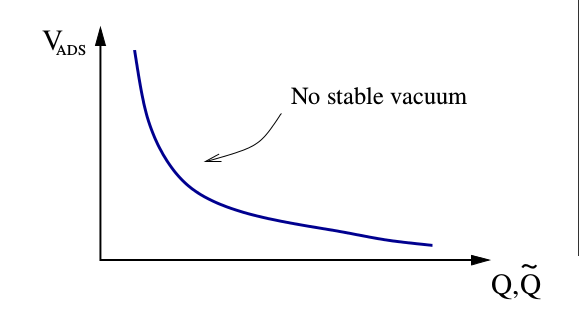
\includegraphics[scale=0.5]{ads_super.png}
\end{center}
This situation is the perfect example where, unlike the classical moduli space, quantum corrections lift completely the moduli space and the theory does not posseses a vacuum anymore.

\paragraph{$\mathbf{ N_f = N_c}$}
When the number of flavours is equal the number of colours of the theory, the classical moduli space was subject to the constraint
\begin{equation}
 \Det{M} - B \tilde{B} = 0
\end{equation}
In the quantum corrected moduli space mesons and baryons satisfy \cite{Seiberg:1994bz}
\begin{equation}
 \Det{M} - B \tilde{B} = \Lambda^{2 N_c}
\end{equation}
which flows to the classical constraint in the classical limit ($\Lambda \; \rightarrow \;0$).
\\
\begin{SCfigure}[1.3][h]
\centering
{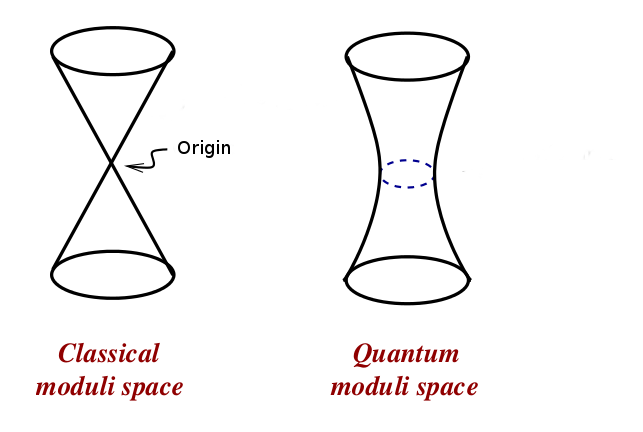
\includegraphics[width=5 cm]{quantum_moduli_space_sqcd.png} }
{\caption{ Quantum and classical representation of the moduli space near the origin}}
\end{SCfigure}
The effect of this relation is that the origin  does not belong to the moduli space anymore and the moduli space is now smooth.
For large expectation values of $M$, $B$ and $\tilde{B}$ the classical and the quantum moduli space look similar, while in the origin of the moduli space quantum corrections modify drastically the structure of the moduli space.
Moreover, the subspace with $B$ or $\tilde{B}$ equal to zero, is not singular anymore while classically the meson matrix was constrained to have zero determinant. 
\\
Because the origin is not in the quantum moduli space the global symmetry group is necessarily broken in some way, depending on the position of the moduli space 
\begin{align}
M^i_j = \Lambda^2 \delta^i_j \quad B=\tilde{B}= 0 \quad & \rightarrow  \quad SU(N_f)_V \times U(1)_B \times U(1)_R\\
\quad M^i_j = 0 \quad B=-\tilde{B}= \Lambda^{N_c} \quad & \rightarrow  \quad SU(N_f)_L \times SU(N_f)_R \times U(1)_R
\end{align}
where $SU(N_f)_V$ is the diagonal vector subgroup.
\\
\paragraph{$\mathbf{N_f = N_c +1}$}
In the case $N_f = N_c +1 $ the classical moduli space is constrained by
\begin{equation}
 \Det{M} \left( \frac{1}{M}\right)^j_i - B_i \tilde{B}^j = 0 \qquad
 M^i_j B_i = M^i_j \tilde{B}^j = 0 
 \label{eqn:N_f__N_c_1_classical_constraints}
\end{equation}
and quantum corrections do not modify it.
In the previous section we noted that the singularities in the classical moduli space are associated to the appearance of massless gluons.
In the quantum picture, the interpretation of the singularities is different: they are associated with additional massless mesons and baryons.
At the origin of the moduli space the theory is strongly coupled and the global symmetry \eqref{eqn:seib_dual_global_symm_group} is unbroken and it can be checked using 't Hooft anomalies \cite{Seiberg:1994bz}.
Far from the origin, the mesons and baryons interact with the potential 
\begin{equation}
W = \frac{1}{\Lambda^{2 N_c -1}} \left( M^i_j B_i \tilde{B}^j - \Det{M} \right)
\end{equation}
that enforce the classical constraints \eqref{eqn:N_f__N_c_1_classical_constraints} through the equations of motion.
For large VEVs of the fields, mesons and baryons acquire large mass through the superpotential.
\paragraph{$\mathbf{ N_f > N_c +1 }$}
Starting from $N_f = N_c +2$ it is not possible to construct a physical superpotential out of gauge invariant operators, in analogy to the previous cases.
The only $SU(N_f)_L \times SU(N_f)_R$ invariant superpotential that can be written is given by
\begin{equation}
 W_{eff} \sim \Det{M} - B_{ij} M^i_k M^j_l \tilde{B}^{kl} 
 \end{equation} 
because baryons have two flavour indices.
However this superpotential does not have R-charge equal to two and if we add more flavours we should add other mesons to the superpotential. Therefore the classical moduli space is not modified by quantum corrections.
As a result, near the origin the quantum corrected moduli space looks identical to the classical one.
Unlike the case with $N_f = N_c +1$ the singularities in the moduli space cannot be interpreted as massless mesons and baryons and an effective description of these operator is singular \cite{Seiberg:1994bz}.
Considering that the 't Hooft anomaly matching conditions are not satisfied in the singular points it is clear that a description using mesons and baryons is not correct.
\\
To find a description of the low-energy degrees of freedom of the theory we will use Seiberg duality, which provides an alternative description of the theory.

\paragraph{\textbf{Conformal window}}
%$\mathbf{  \frac{3}{2} N_c \geq N_f \geq  3 N_c}$ \textbf{: the conformal window}\\
Thetheory is not asympotically free in the range $\frac{3}{2} N_c < N_f < 3 N_c$. This can be seen by using the \emph{NSVZ} $\beta$ function\eqref{eqn:suN_Dynkin_indices}, which reads
\begin{align}
 \beta (g) & \, = \,- \frac{g^3}{16 \pi^2} \frac{3 N_c - N_f + N_f \gamma(g^2)}{1 - N_c \frac{g^2}{8 \pi^2}} \\
\gamma(g^2) &  \,= \, - \frac{g^2}{8 \pi^2} \frac{N_c^2 - 1}{N_c} + \mathcal{O} (g^4)
\end{align} 
The $\beta$ function is known to have a Banks-Zaks fixed point \cite{Banks:1981nn} in the 't Hooft limit with $\frac{N_f}{N_c} = 3 - \epsilon$ held fixed and $\epsilon \ll 1$.
However, the fixed point exists in the range of values $\frac{3}{2} N_c \geq N_f \geq  3 N_c$ with $N_f$ and $N_c$ finite.
This is possible because one loop and two loop contributions to the beta function have opposite signs.
As a result, the infrared theory is a non-trivial four dimensional superconformal theory. 
The infrared degrees of freedom are quarks and gluons that are not confining but are interacting as massless particles.
The theory is in a free non-Abelian Coulomb phase.
\\
The fact that the theory is superconformal implies that we have further restrictions on the algebra of operators \footnote{
	R-symmetry is part of the superconformal algebra instead of being an automorphism of the algebra, as in superPoincarè algebra.  
	}.
Superconformal algebra imposes that the dimension of every operator satisfy this inequality involving the R-charge
\begin{equation}
 D \geq \frac{3}{2} \; | R |
 \label{eqn:superconformal_dimension_rcharge}
\end{equation}
where the bound is satured for chiral fields.\\
The product of two chiral operator is constrained by this fact.
%Because $R( O_1 O_2) = R(O_1) + R(O_2)$, for chiral operators, which saturate the bound \eqref{eqn:superconformal_dimension_rcharge}, $D(O_1 O_2) = D(O_1) + D(O_2)$. 
Consider that for two operators $O_1,O_2$ we have $R( O_1 O_2) = R(O_1) + R(O_2)$.
Because of the bound \eqref{eqn:superconformal_dimension_rcharge}, the scaling dimension of chiral operators is additive $D(O_1 O_2) = D(O_1) + D(O_2) = \frac{3}{2} R(O_1) + \frac{3}{2} R(O_2)$.
Note that the dimension of the operator is quantum corrected, i.e. contains the anomalous dimension of the operator.
%Therefore, the OPE is not singular and the product of operators is well-defined. Because of this fact, chiral operators form the \emph{chiral ring}. 
\\
Given that the superconformal R-symmetry is not anomalous and commutes with the global symmetry group of the theory, then it must be the R-symmetry that appears in table \ref{tab:suN_elect_charge}.
Because of \eqref{eqn:superconformal_dimension_rcharge}, the gauge invariant operators we defined previously must have the following dimensions
\begin{align}
 D(Q \tilde{Q}) &= \frac{3}{2} R(Q \tilde{Q}) = 3 \frac{N_f - N_c}{N_f}\\
 D(B) & = D(\tilde{B})  = \frac{3}{2} N_c \frac{N_f - N_c}{N_c}
\end{align}
\\
Gauge invariant operators should be in unitary representation of the superconformal algebra.
Unitarity imposes that in general $D\geq 1$ and the equality holds for singlet fields.
From the previous equation we can verify that $D(M) \geq 1$ for $ N_f \geq \frac{3}{2}N_c$ and it becomes a free field for $N_f = \frac{3}{2}N_c$. 
\\
For fewer number of flavours, the meson field is inconsistent with the unitarity bound.
The theory is conjectured to flow to a different phase.
\\
\paragraph{$\mathbf{ N_f > 3 N_c}$}
In this range, quarks prevails on gluons and change the sign of the $\beta$ function. 
This is caused by the \emph{charge screening} effect of quarks, that make the coupling constant smaller at larger distances.\\
The theory is in a free non-Abelian electric phase.
Its behaviour is not well defined at high energies because of the presence of a Landau pole at $R \sim \Lambda^{-1}$, although the theory can be a good description of a low-energy limit of another theory. 





















\subsection{Magnetic theory}
The magnetic theory is a \emph{SQCD} theory with the same global symmetries as the electric theory, but with gauge group $SU(N_f - N_c)$. 
In addition there are $N_f^2$ color singlets, that we will call mesons, Considering that they have the same properties as the mesons we can construct in the electric theory.
In the magnetic theory they are fundamental fields i.e. they are not written as gauge invariant operators from quarks. 
Given that they are gauge invariant, they interact only through the superpotential
\begin{equation}
 W  = M^i_{\tilde{j}} \; q_i \, \tilde{q}^{\tilde{j}}
 \label{eqn:seiberg_duality_mag_super}
\end{equation}
where we represented dual quarks as $q,\tilde{q}$ and mesons as $M^i_{\tilde{j}} $.\\
The charges of fields of the magnetic theory are
\begin{equation}
 \begin{array}{| c | c |  c c c c |  }
 \hline
 & SU(N_c) & SU(N_f)_L  &SU(N_f)_R   & U(1)_B &  U(1)_R \\
\hline
q & N_c & \overbar{N_F} & 1   &   \frac{N_c}{N_f-N_c}   &  \frac{N_c}{N_f}  \\
\tilde{q} &\overbar{N_c}  &  1 & { N_F}   & - \frac{N_c}{N_f-N_c}   &   \frac{N_c}{N_f}   \\	 
M^i_{\tilde{j}}  &  1  & N_f & \overbar{N_f}  & 0 &  2 \frac{N_f - N_c}{N_f}\\ 
\hline
 \end{array}
 \label{tab:sun_magnetich_charges}
	%\centering
 %\caption{Charges of the magnetic theory}
\end{equation}\\
Dual quarks are in opposite representation of flavour symmetries. 
\\
Mesons in the magnetic theory have the same charges of the mesons constructed from electric quarks.
Baryons constructed from dual quarks have the same baryonic charge as the electric baryons and are mapped into each other by the duality.
It can be demonstrated that they are proportional to each other.\\
Similarly to the electric theory, the R-charges can be chosen in order for the R-symmetry to be non-anomalous.\\
However, the R-charges can be found by imposing the duality.
If we use the fact  that the mesons are built from electric quarks, their R-charge is twice the R-charge of electric quarks.
The R-charges of the dual quarks can be found by imposing that the term $M q \tilde{q}$ of \eqref{eqn:seiberg_duality_mag_super} has R-charge two.
In this way, we found the R-charges at the superconformal infrared fixed point.



\subsubsection{Phases of the magnetic theory}
In order to study the phases of the dual theory we can map the various ranges of flavours of the electric theory into ranges for the magnetic theory by considering the relation $\tilde{N_c} = N_f - N_c$
\begin{equation}
\begin{array}{c  c  c  c}
%& & &  \lj
\hbox{Electric} & N_c +2 \leq N_f \leq \frac{3}{2}N_c &  \frac{3}{2}N_c  < N_f < 3 N_c & N_f \geq 3 N_f \\[3mm]
\hbox{Magnetic} & N_f \geq 3 N_c  &  \frac{3}{2}N_c  < N_f < 3 N_c &  N_c +2\leq N_f \leq \frac{3}{2} N_c  \\[2mm]
\end{array}
\end{equation}
As we can see from the table, both the electric and magnetic theories are in the conformal windows for the same values of $N_f,N_c$.
In the other two intervals, the dual theories are in opposite phases.
\\
For $N_c +2 \leq N_f \leq \frac{3}{2} N_c$ the electric theory is strongly coupled and we can't describe its dynamics. 
On the other hand, the magnetic theory is free and can be used to describe the physics for this range of flavours.\\
When the electric theory is in a free non-Abelian phases ( $N_f \geq 3 N_c$), the magnetic theory is strongly coupled.\\
This feature of Seiberg duality is particularly useful, because it gives us a weakly coupled description of a strongly-coupled theory.  





\subsubsection{Duality}
In the \emph{conformal window} the electric and magnetic theories we introduced previously give an equivalent description of the same physics in the infrared.
In this range, the magnetic theory has a non-trivial infrared fixed point too. 
At this fixed point, the superpotential \eqref{eqn:seiberg_duality_mag_super} is a relevant perturbation because it has dimension $D = 1 + 3 \frac{N_c}{N_f}  <3 $ and it drives the theory to a new fixed point.\\
Electric mesons have different dimension in the UV from the magnetic ones because they are constructed from a pair of quark.
For this reason it is necessary to introduce an energy scale $\mu$ in order to match their dimension in the UV: $ M = \mu M_m$, where $M_m$ are the magnetic mesons.\\
The matching of the scales between the electric and mangetic theory results in the following relation between them \cite{Seiberg:1994pq}
%The strong coupling scales of the electric $\Lambda$ and magnetic $\tilde{\Lambda}$ theories are related by the relation
\begin{equation}
 \Lambda^{3 N_c - N_f} \tilde{\Lambda}^{3 (N_f - N_c) - N_f} = (-1)^{N_f - N_c} \mu^{N_f}
 \label{eqn:seib_dual_matching_scales}
\end{equation}
This relation shows that when one theory is strongly coupled, the other is weakly coupled.
Moreover, it ensures that the dual of the dual theory is the electric theory itself.
The dual of the dual magnetic theory is a $SU(N_c) $ \emph{SQCD} theory with scale $\Lambda$, $d^i$ and $\tilde{d}_{\tilde{j}}$ quarks and additional singlets $M^i_{\tilde{j}}$ and $N^{\tilde{j}}_i= q_i q^{\tilde{j}} $ with superpotential
\begin{equation}
 W = \frac{1}{\tilde{\mu}} N^{\tilde{j}}_i d^i \tilde{d}_{\tilde{j}} + \frac{1}{\mu} M^i_{\tilde{j}} N^{\tilde{j}}_i = \frac{1}{\mu} N^{\tilde{j}}_i \left(  - d^i d_{\tilde{j}}  + M^i_{\tilde{j}}  \right) 
\end{equation}
considering that from the previous relation we have $\tilde{\mu} = - \mu$.\\
Meson fields are massive and can be integrated out by using their equation of motion,which result in
\begin{equation}
 N^{\tilde{j}}_i  = 0 \qquad  M^i_{\tilde{j}} = d^i d_{\tilde{j}}
\end{equation}
Given that the dual theories describe the same physics, there should be a mapping of gauge invariant operators between them.
We already saw that electric and magnetic mesons match in the infrared. 
A mapping should exists also for baryonic operators. Indeed it does and it is given by
\begin{equation}
\begin{aligned}
 B^{i_1 \dots i_{N_c}} & = C \; \epsilon^{i_1 \dots i_{N_c} j_1 \dots i_{N_f - N_c}} b_{j_1 \dots j_{N_f - N_C}}\\
 \tilde{B}^{i_1 \dots i_{N_c}} &= C \; \epsilon_{\tilde{i}_1 \dots \tilde{i}_{N_c} \tilde{j}_1 \dots \tilde{i}_{N_f - N_c}} b_{ \tilde{j}_1 \dots \tilde{j}_{N_f - N_C}}\\
 \text{where} \qquad C & = \sqrt{ - (-\mu)^{N_c - N_f} \Lambda^{3 N_c - N_f}}
\end{aligned}
\end{equation}
using \eqref{eqn:seib_dual_matching_scales} it can be shown that these mappings preserve the involutive action of the duality. 

As an additional check of the duality, 't Hooft anomaly matching conditions have been calculated  in \cite{Seiberg:1994pq} for the electric and magnetic theories for the various global symmetries and in both theories they are given by
\begin{equation}
\begin{aligned}
SU(N_f)^3 \quad \longrightarrow \quad   & N_c \\
U(1)_R\, SU(N_f)^2 \quad \longrightarrow \quad  & -\frac{N_c^2}{2 N_f} \\
U(1)_B\, SU(N_f)^2 \quad \longrightarrow \quad  & \frac{N_c}{2} \\
U(1)_R \quad \longrightarrow \quad  & -N_c^2 - 1 \\
U(1)_R^3 \quad \longrightarrow \quad  & -N_c^2 - 1 - 2 \frac{N_c^4}{N_f^2} \\
U(1)_B^2 U(1)_R \quad \longrightarrow \quad  & - 2 N_c^2 \\
\end{aligned}
\end{equation}
Another important check of the duality is that it remains valid under mass perturbations of the electric theory.
Suppose to add a superpotential term that gives mass to the quark in the last flavour and is equal to
\begin{equation}
	W_{mass}^{el} = m \; Q_{N_f} \tilde{Q}^{N_f}
\end{equation}
Flowing to the IR the number of quarks is decreased by one, driving the theory to a more strongly coupled fixed point\footnote{Considering that matter in the fundamental representation contributes with a positve term it is easy to see that this is true.}.
The new scale of the theory is given in terms of the old one by
\begin{equation}
 \Lambda_{L}^{3 N_c - (N_f - 1)} = m \; \Lambda^{3 N_c - N_f}
\end{equation}
In the magnetic theory the mass perturbation is mapped in the term
\begin{equation}
W_{mass}^{mag} = m \; M_{N_f}^{N_f}
\end{equation}
Because of this term, the gauge group gets higgsed to $SU(N_f-1 - N_c)$ and only $N_f -1$ light quarks remain in the theory. \\
The scale of the magnetic theory $\Lambda_L$ is modified and reads
\begin{equation}
\tilde{\Lambda}^{3(N_f - N_c -1) - (N_f -1)} = 
- \frac{
	\tilde{\Lambda}^{3 (N_f - N_c) - N_f}	
	}
	{
	< q_{N_f} \tilde{q}^{N_f}		>
	}
\end{equation}
where $< q_{N_f} \tilde{q}^{N_f}> = - \mu m $ because of the equation of motion for the massive flavour. \\
As expected the magnetic theory becomes more weakly coupled.\\
We conclude that the duality is preserved under massive deformations.  